% Created 2021-05-07 Fri 11:54
% Intended LaTeX compiler: pdflatex
\documentclass[9pt, b5paper]{article}
\usepackage[UTF8]{ctex}
\usepackage{fontspec}
\usepackage{graphicx}
\usepackage{xcolor}
\usepackage{multirow}
\usepackage{multicol}
\usepackage{float}
\usepackage{textcomp}
\usepackage{geometry}
\geometry{left=1.2cm,right=1.2cm,top=1.5cm,bottom=1.2cm}
\usepackage{algorithm}
\usepackage{algorithmic}
\usepackage{latexsym}
\usepackage{natbib}
\usepackage{listings}
\usepackage{minted}
\usepackage[xetex,colorlinks=true,CJKbookmarks=true,linkcolor=blue,urlcolor=blue,menucolor=blue]{hyperref}
\author{deepwaterooo}
\date{\today}
\title{成长的故事——我和表哥}
\hypersetup{
 pdfauthor={deepwaterooo},
 pdftitle={成长的故事——我和表哥},
 pdfkeywords={},
 pdfsubject={},
 pdfcreator={Emacs 27.1 (Org mode 9.3)}, 
 pdflang={English}}
\begin{document}

\maketitle
\tableofcontents


\section{2013 Summer Intern 暑假实习(2) ——}
\label{sec:orgee1c263}

\begin{center}

\includegraphics[width=.9\linewidth]{/Volumes/f/kcwang/pic/backups_plans_20210507_091504.png}
\end{center}

前面说到,当我的小导师不专业的作风把自己激怒,当我在自己的小导师的座位指出她的一个bug,当组长C极力为她扫地,为她安排一个所谓的彰显个人能力的所谓的报告,而我又不去参加的时候,办公室的氛围把人整疯了!

\begin{center}

\includegraphics[width=.9\linewidth]{/Volumes/f/kcwang/pic/backups_plans_20210507_091648.png}
\end{center}

那天,我被办公室里的气氛搞疯了,躲在厕所里哭了。 

\begin{center}
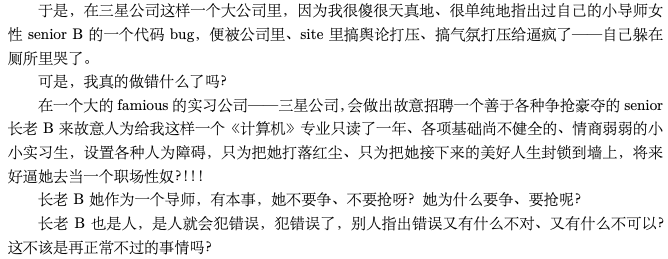
\includegraphics[width=.9\linewidth]{/Volumes/f/kcwang/pic/backups_plans_20210507_091755.png}
\end{center}

\begin{center}
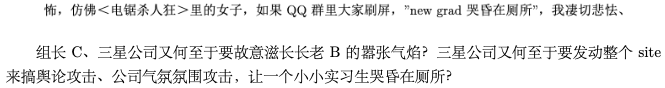
\includegraphics[width=.9\linewidth]{/Volumes/f/kcwang/pic/backups_plans_20210507_091828.png}
\end{center}

那个女的发邮件,把表姐和我的名字写到最后

写大表姐是如何被招入三星的,

\begin{center}

\includegraphics[width=.9\linewidth]{/Volumes/f/kcwang/pic/backups_plans_20210507_092305.png}
\end{center}

表姐感受到压力,便周末拉我陪理道歉!

\begin{center}

\includegraphics[width=.9\linewidth]{/Volumes/f/kcwang/pic/backups_plans_20210507_092433.png}
\end{center}

这个歉我道得是心不甘、情不愿,只是迫于大表姐的压力,才不得不装装样子

\begin{center}

\includegraphics[width=.9\linewidth]{/Volumes/f/kcwang/pic/backups_plans_20210507_092526.png}
\end{center}

解决问题的根本原因是什么呢?是大家各自心底对自己工作的来历的感激

大神长老B的过往?《要在这里写吗?》

\begin{center}

\includegraphics[width=.9\linewidth]{/Volumes/f/kcwang/pic/backups_plans_20210507_092150.png}
\end{center}

大表姐的索要回报?


\begin{center}

\includegraphics[width=.9\linewidth]{/Volumes/f/kcwang/pic/backups_plans_20210507_092117.png}
\end{center}

写我自己的锻炼身体《交待背景》交待十年前情敌的前后文

\begin{center}

\includegraphics[width=.9\linewidth]{/Volumes/f/kcwang/pic/backups_plans_20210507_091150.png}
\end{center}

实习的重点:考验人际关系、情商测试

\begin{center}

\includegraphics[width=.9\linewidth]{/Volumes/f/kcwang/pic/backups_plans_20210507_093408.png}
\end{center}

大表姐要求后,我表现出真正的真诚

当我近乎讨好、打趣儿自己的小导师、长老B说,“那你明天要不要带上我去给你当小秘呀?!”之后,其它人是什么反应呢?

\begin{center}

\includegraphics[width=.9\linewidth]{/Volumes/f/kcwang/pic/backups_plans_20210507_093537.png}
\end{center}

这些都是职场里的人际关系!

你以为我做得很好?错了,实习后期、最后两个周的人际关系直接就把人给搞疯了、搞崩溃了!

\begin{center}
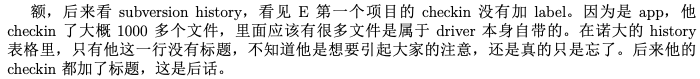
\includegraphics[width=.9\linewidth]{/Volumes/f/kcwang/pic/backups_plans_20210507_095519.png}
\end{center}

写实习生E也提交了一个项目 

这里也暂时来回顾一下这内个周里我们实习生E的表现吧

当我无视组长C为长老B的出风头的会议的时候,实习生E是如何表现的呢?

\begin{center}

\includegraphics[width=.9\linewidth]{/Volumes/f/kcwang/pic/backups_plans_20210507_095110.png}
\end{center}

\begin{center}

\includegraphics[width=.9\linewidth]{/Volumes/f/kcwang/pic/backups_plans_20210507_095131.png}
\end{center}

E也是直接如我般没有去参加长老B的会议的!实习生E是加入了我的一侧、相当于是直接参与煽风点火、煽动捣乱!组长C的管理确实不给力呀。 

\begin{center}
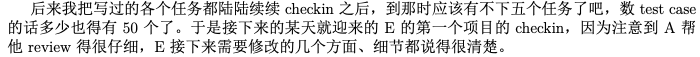
\includegraphics[width=.9\linewidth]{/Volumes/f/kcwang/pic/backups_plans_20210507_094737.png}
\end{center}

恩,他们正式员工忙他们的,我们小兵玩儿我们的!

\begin{center}

\includegraphics[width=.9\linewidth]{/Volumes/f/kcwang/pic/backups_plans_20210507_104400.png}
\end{center}

我请实习生E帮我demo一下他提交的他的第一个项目

\begin{center}
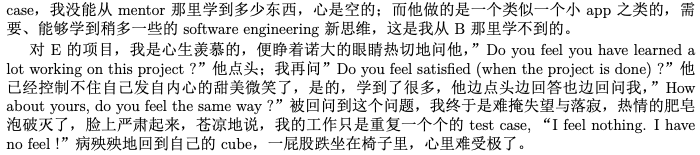
\includegraphics[width=.9\linewidth]{/Volumes/f/kcwang/pic/backups_plans_20210507_104525.png}
\end{center}

这是自己的一种渴求的表达,实际上当初正式员工A有发python的链接给我,其实也早就说明了我是早晚还是会、能够从正式员工A那里学些东西的,不是吗?

\begin{center}

\includegraphics[width=.9\linewidth]{/Volumes/f/kcwang/pic/backups_plans_20210507_104827.png}
\end{center}

办公室里的氛围应试是证实当初实习公司确实有过这种打算和安排吧。 

那么,他们要先按排长老B作为我的实习生的原因、和目的又是什么呢?

\begin{center}

\includegraphics[width=.9\linewidth]{/Volumes/f/kcwang/pic/backups_plans_20210507_105100.png}
\end{center}

refer实习生E进公司的(据说是E的舅舅)board里的老K坐到我们餐桌上的目的是什么呢?进一步的昭明公司里对我打压的态度?!!!

\begin{center}

\includegraphics[width=.9\linewidth]{/Volumes/f/kcwang/pic/backups_plans_20210507_105255.png}
\end{center}

这些是那件事的后述。当时的自已还是比较幼稚的,再成熟一点儿,他老K说他的,关我什么事儿吗?我该干嘛照样干嘛,只不把你当回事儿便是了。 

\begin{center}
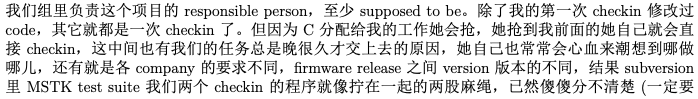
\includegraphics[width=.9\linewidth]{/Volumes/f/kcwang/pic/backups_plans_20210507_093941.png}
\end{center}

这时项目中存在的问题:subversion傻傻分不清楚

\begin{center}

\includegraphics[width=.9\linewidth]{/Volumes/f/kcwang/pic/backups_plans_20210507_094042.png}
\end{center}

这个,就太不像话了呀

\begin{center}
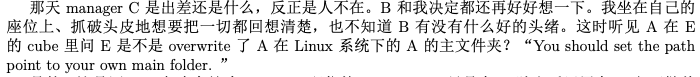
\includegraphics[width=.9\linewidth]{/Volumes/f/kcwang/pic/backups_plans_20210507_094121.png}
\end{center}

\begin{center}

\includegraphics[width=.9\linewidth]{/Volumes/f/kcwang/pic/backups_plans_20210507_094251.png}
\end{center}

当时,我只看见了这个在组长C缺席的时候,正式员工A为平衡组里的关系所做出的一点儿小小平衡

当时的自己却没有想明白,与长老B的项目像两股拧在一起的麻绳,傻傻分不清楚,应该是需要我自己建一个自己的文件夹的!但当时的自己竟然是没有听明白!

当时的我没有听明白,当时的我自己也不明白,这个暑假是一定会被他们搞死的,一如现在长老B就是故意各种不教自己、各种给自己添乱,一如尖人一早就给我的专业能力石头打压!!!

尖人的定调:这个假期就是要搞倒你\textasciitilde{}! <这里写到哪里才比较好呢?把这个定调找一个相对比较好的地方>

\begin{center}

\includegraphics[width=.9\linewidth]{/Volumes/f/kcwang/pic/backups_plans_20210507_091356.png}
\end{center}

而我当时的反应是: 

\begin{center}

\includegraphics[width=.9\linewidth]{/Volumes/f/kcwang/pic/backups_plans_20210507_091418.png}
\end{center}

尖人是一个什么样的人呢?

\begin{center}

\includegraphics[width=.9\linewidth]{/Volumes/f/kcwang/pic/backups_plans_20210507_103838.png}
\end{center}

尖人的定调:这个假期就是要搞倒你\textasciitilde{}!

\begin{center}

\includegraphics[width=.9\linewidth]{./pic/backups_plans_20210424_215822.png}
\end{center}

为自己争credit的欲望在增强!<可以用在以后的什么地方>

当正式员工站出来平衡一下组里的关系,为什么尖人就怎么呢?

\begin{center}

\includegraphics[width=.9\linewidth]{/Volumes/f/kcwang/pic/backups_plans_20210507_103521.png}
\end{center}

为什么尖人和实习生E要一定向正式员工A问一些关于God的问题呢?

这两个狡诈的人,走的便是公司里早已布局、也已(逼良为娼产业链实习情商测试工厂)成型的对职场新人的情商测试,虽然当时的当事人——我亲爱表哥眼中的少女心小弱弱并不知晓这一点儿、浑然不觉!

话说尖人,恩,尖人,总是这么地察颜观色,并实时实行精准打击!

\begin{center}

\includegraphics[width=.9\linewidth]{/Volumes/f/kcwang/pic/backups_plans_20210507_105925.png}
\end{center}

你看,长老B这会儿不是正在教我么,接下来便是,组长C说她要下周出差!好准好巧哦!

\begin{center}
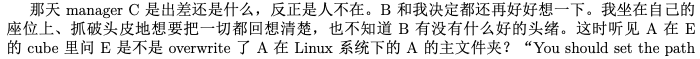
\includegraphics[width=.9\linewidth]{/Volumes/f/kcwang/pic/backups_plans_20210507_110205.png}
\end{center}

上次是什么情况,组长C偏巧不在,正式员工A说了那么一句话,便被公司的里的一两只警犬往偏路上去推和逼!

那么当组长C要出差,当自己的小导师senior长老B累积了、被组长C问起了他那成堆的Bug要怎么办时,我是怎么做的呢?

\begin{center}
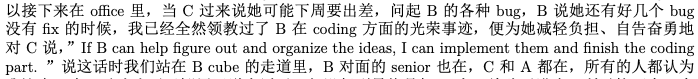
\includegraphics[width=.9\linewidth]{/Volumes/f/kcwang/pic/backups_plans_20210507_110401.png}
\end{center}

我认为自己能够承担和愿意付出努力的便是:在自己当时的小导师、长老B的修改bug的思想指导下,我可以实现所有的代码部分(代码的实现完成与机器测试通过)。我认为这是自己力所能及、可以做得到、并且应该主动承担的(实习生的责任)! 

当年那个《计算机》专业只读、只学习了一年的小弱弱,她的这份自信心、在工作需要面前、在这诸多的正式员工面前,敢于承担责任的责任心、或是更确切地说,自信心,源自于哪里???

\begin{center}

\includegraphics[width=.9\linewidth]{./pic/backups_plans_20210502_114726.png}
\end{center}

我写过Tic-Tac-Toe的一步move;

\begin{center}

\includegraphics[width=.9\linewidth]{./pic/backups_plans_20210502_120523.png}
\end{center}

\begin{center}

\includegraphics[width=.9\linewidth]{/Volumes/f/kcwang/pic/backups_plans_20210507_111947.png}
\end{center}

我早前这年2月14日情人节、写出过密码设置为要我亲爱的表哥爱我一世(2514)的RTOS(实时操作系统)作业!

\begin{center}

\includegraphics[width=.9\linewidth]{/Volumes/f/kcwang/pic/backups_plans_20210507_111500.png}
\end{center}

这个春季学期快要结束的时候,我也写出过AI(Artifical Intelligence人工智能)课decision tree的项目,那种 \textbf{能够把自己跃跃欲试、心里想往的事情做好,这种感觉真的狠好!}

\begin{center}

\includegraphics[width=.9\linewidth]{/Volumes/f/kcwang/pic/backups_plans_20210507_112714.png}
\end{center}

我又过了三天两早上、尾巴又开始跷起来了、又说大话了吗?

我只是一个个小小实习生,对三星公司的硬件产品SSD我并没有足够的了解和信心,所以,我没有能力和信心,我还做不到 \textbf{独立} 完成这所有长老B所遗留下来的test case bugs的修复。

我自认为自己没有说大话。

\begin{center}

\includegraphics[width=.9\linewidth]{/Volumes/f/kcwang/pic/backups_plans_20210507_110611.png}
\end{center}

组长C周五离开前写邮件给长老B和我:要我debug B之前项目中留下来的5个test case bugs \textbf{under B's gidence} .

我因为曾经的、能够把自己跃跃欲试、心里想往的事情做好的感觉狠好,而主动承担了这次接下来一周的test case bugs修复事件的代码实现与测试,那我这次还能够把自己心里想往的事情做好吗?我还能重复、再次建立和巩固这个专业里的小弱弱的心里想往与自信心吗?

但结果是这次bugs修复测试事件,我正当防卫没把自己陷进去,却把长老B她自己(是她自己的项目)给陷进了舆论的漩涡里,公司里出了很大的力、宏观调控与布署才再得以平复。

\begin{center}

\includegraphics[width=.9\linewidth]{/Volumes/f/kcwang/pic/backups_plans_20210507_113912.png}
\end{center}

5个test case,简单的、容易的四个上斑第一天我就做完了。 

\begin{center}

\includegraphics[width=.9\linewidth]{/Volumes/f/kcwang/pic/backups_plans_20210507_114031.png}
\end{center}

但是还剩下一个难的,就成为了第二天、那个周二我的山大压力!

\begin{center}

\includegraphics[width=.9\linewidth]{/Volumes/f/kcwang/pic/backups_plans_20210507_114156.png}
\end{center}

那个bug到底算是怎么回事呢?

\begin{center}

\includegraphics[width=.9\linewidth]{/Volumes/f/kcwang/pic/backups_plans_20210507_114437.png}
\end{center}

这时请注意,当年我写“我找不到现有的例子”,不是像实习第一个小项目,我从长老B所写过的test case里找找参考例子,而是从整个site里,从整个MSTK测试项目里去找,也找不到能够用来参考的例子。 

\begin{center}
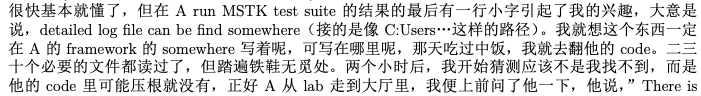
\includegraphics[width=.9\linewidth]{/Volumes/f/kcwang/pic/backups_plans_20210507_115308.png}
\end{center}

\begin{center}
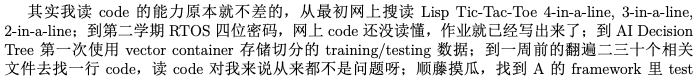
\includegraphics[width=.9\linewidth]{/Volumes/f/kcwang/pic/backups_plans_20210507_115147.png}
\end{center}

这里也再强调一下,当时自己读代码的能力还是不错的了,就是确实从那个项目里找不到那两个(logSense(args), logCommand(args))任何一个样关命令的调用方法。

\begin{itemize}
\item 把小导师当成记忆深处那个:
\item 穿着白色T恤我感觉表哥穿得很fit/我看着很舒服的、看得好养眼看到好舒服只想求抱抱的我亲爱的表哥,身材身形都极好、很完美的我的表哥;
\item 理想里、脑海中、写给我的邮件里对我的职场工作有着有过清晰地表达、职场工作中也一定是意气风发形象的表哥
\item 合二为一

CS570:穷凶极恶
什么情况下穷凶极恶比较好,什么情况下是不可以的?
好坏都对比一下

追忆RTOS2514的作业,为什么不是自己一行一行写出来的代码呢?

不是说第一学期上到一半、一大半的时候终于可以开始自己想问题、自己编代码了吗?为什么第二学期了还在抄网上的代码,并且而以此而洋洋自得呢?!!!

E说大的程序他调不出来的时候,为什么我会有着强大本能的自信来反驳他?为什么那个夏天我就那么自信呢?

对于RTOS课,上面的这种情况只是在自己能够真正写得出作业的时候,可是当自己的代码存在问题的时候,我还能如此顺利吗?

\begin{center}
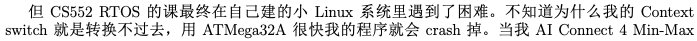
\includegraphics[width=.9\linewidth]{./pic/backups_plans_20210424_215728.png}
\end{center}

\begin{center}
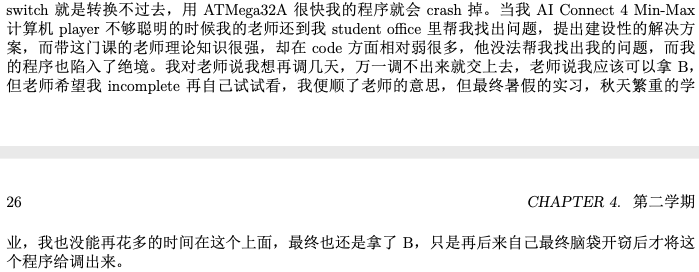
\includegraphics[width=.9\linewidth]{./pic/backups_plans_20210424_215743.png}
\end{center}

对于不能很好地指导自己的导师,在自己遇到困难的时候,得不到应有的帮助,而我又还没能学会真正自己解决问题的时候,还真的是好无力!
\end{itemize}


\section{读计算机专业时的必要大事记:每个学期上万块钱的学费只给选7个学分,我是接受不了的,我没有那么大的经济实力《已经写了》}
\label{sec:orgaba91f1}
\begin{itemize}
\item 本系大牛对于速读速毕业的转专业(大龄)学生的做法与认可度
\begin{itemize}
\item 本系大牛对于推进广大学生朋友、国际留学生婚姻婚事的做法
\end{itemize}
\item 集中在一个学期,大家都结婚了:大牛自己的女博士生也是等了好几年一直等到这个特定的时期才写学校里众多的国际留学生一个夏天结的婚
\begin{itemize}
\item 本系对于国际留学生专业方向的推向(把另一个大25岁马推到这里来)??? —— 要写吗,与表哥舅舅学校的比起来呢
\item 毕业时系里方面有劝过的读博士的可能性,他们说:如果我读博士,如果我不喜欢表哥,我可以不用嫁给他;他们居然不知道我从来都是真心喜欢我表哥的
\end{itemize}
\end{itemize}
(一定要把那个单词找出来,并真正找出它的意思来,并明白它的意思到底是什么,狠重要)!
\subsection{其它(可要可不要)}
\label{sec:org4d6a228}
自己导师罪恶行径的两手准备,并准备发动力量来封死这么一个国际留学生
系里大牛的态度: honolulu
\begin{center}

\includegraphics[width=.9\linewidth]{./pic/backups_plans_20210424_215120.png}
\end{center}
\begin{center}

\includegraphics[width=.9\linewidth]{./pic/backups_plans_20210424_215147.png}
\end{center}
唐立淇:神等级的专业
2014年夏天自己出来写之后的风暴:
那么当时王夏华的出发点到底是受控于三星公司,为接下2015年他们公司的炒作提供支持呢?
还是听从于当时另一派的指挥,以至于最即我能够及时地将两年、尤其是去年暑假的实习写出来?
于是一场实习,卷了一场风暴,迷糊打趴了自己,也伤及周围所有的其它人?
\subsection{那个年代的小伙伴: 闺密、板块与我:竞争与友情?}
\label{sec:org6c70161}
选择困难症:我不是
\begin{center}

\includegraphics[width=.9\linewidth]{./pic/backups_plans_20210422_100215.png}
\end{center}
\begin{center}
\includegraphics[width=.9\linewidth]{./pic/backups_plans_20210422_110112.png}
\end{center}
\begin{center}
\includegraphics[width=.9\linewidth]{./pic/backups_plans_20210422_110135.png}
\end{center}
\subsection{向上的蜗牛}
\label{sec:orgb19ea2f}
陪导师走路:第一次,你要学会平衡与取舍!
就像当年那想要逃脱牢笼的小鸟,拼了命也想要飞出去,却不知道飞出去的命运究竟是什么呢?
把 《燃情岁月》的结尾
与自己和表哥的经历结合起来,购造一个故事情节、人物性格完整版本的 《燃情岁月》
18年当我的职场生涯遭到封杀后,我于6月份有回中国五个月大概半年的时间,在中国上海的几家小公司工作过。 简述一下当时的情形。
11月我从中国回来。在Palo Alto照顾一位老爷爷。
三大通过网上提醒牙医女儿调整用药的目的,最终我也失去了那份工作。 
这是一种经济上的管控。
具体的事件:老科、肥东,他的朋友圈都转换成了三大的托儿
肥东,赌场里的各种托儿
2015年,赌博输掉了他一年的全部工资。
当年的住处、尘世里自己所嫁的这个人本人已经是一个三大的托儿的存在,那我还有什么好留恋?他不是所有的立场都说明了一切吗?
\subsection{健康问题}
\label{sec:org53cd542}
\begin{center}
\includegraphics[width=.9\linewidth]{./pic/backups_plans_20210424_212545.png}
\end{center}
\begin{center}
\includegraphics[width=.9\linewidth]{./pic/backups_plans_20210424_220817.png}
\end{center}
早上
\begin{center}
\includegraphics[width=.9\linewidth]{./pic/backups_plans_20210424_212910.png}
\end{center}
十二月的一次: 对自己病情的把握与进展的信心

\section{三大炒作网红、逼良为娼洗脑记(3):夏安:职场结局:被逼性奴}
\label{sec:orgf3a8e74}
\begin{itemize}
\item 三大自导自演炒作出的自家网红的结局预告:专业职场的、非专业职场的将来被逼性奴 2014年7月夏安的预告
\begin{center}
\includegraphics[width=.9\linewidth]{./pic/p2p201.png}
\end{center}
\end{itemize}
问号争当版主,与大主力的转移;用《金瓶梅》给被逼当事人洗脑

\section{行走在《计算机》专业的大道上(4)——第三学期}
\label{sec:org5806a41}

\begin{center}
\includegraphics[width=.9\linewidth]{./pic/backups_plans_20210424_213118.png}
\end{center}

\begin{center}
\includegraphics[width=.9\linewidth]{./pic/backups_plans_20210424_213150.png}
\end{center}

第二学期的病情

<第三个学期>  食堂虚脱:没有人情,累死你也要把你放到最后一个去吃饭

\begin{center}
\includegraphics[width=.9\linewidth]{./pic/backups_plans_20210424_095434.png}
\end{center}

<第三个学期>  有一次食堂里虚脱了:写食堂里工作人员的无情:<第三个学期>

  \begin{center}
\includegraphics[width=.9\linewidth]{./pic/p1p136-5.png}
\end{center}
2015年毕业时:读博士与否:一个负责任的做法到底应该是怎样的呢?

\section{另一份专业相关的工作——2017年夏秋季节}
\label{sec:org758663a}
\begin{itemize}
\item 对于紧急事件的处理:被逼性奴怀孕,三大黑势力的处理办法:用一份工作确保被逼当事人不会把小孩生下来(会降低他们手上女色资源的价值、他们拿不到手好回报)、
\end{itemize}
并想尽办法使他们的被逼当事人——不会再怀孕
也写职场上的友情Randy,老板Andy
\begin{itemize}
\item 后续:相关部门工作人员来作报告,我眼神传达报告女士我确实是在被他们一直逼
\item 2月我自己辞职
\item 舅舅喊停: 舅舅也是跟着三大的风向,踩着点儿地喊停的吗?舅舅为什么踩着时间点喊停分析
\end{itemize}

\section{职场生涯(专业职场、非专业相关职场)中的性骚扰}
\label{sec:orgd8967a4}
\begin{itemize}
\item 个人个性中对于界限的认定:个性中对男女有别等的界定与认知
\item 2013年三星实习时那个星期五,问A为什么昨天不能告诉我我的新项目是什么,对于IPO是否会给我OPT延期的这种问话上的清楚与潜意识里的不清醒:
\item \textbf{若明若暗、似有若无的潜意识} 神乎其神的潜意识:可以来个合集
\end{itemize}
以及沉溺环境下长大的、没有经过时间沉淀时、认识事物的反复

\section{离职后的非专业相关硅谷生活,简略快结束}
\label{sec:orga743101}
三大的黑:他们黑我的时候,一如当年他们会故意禁网,故意制造人民群众不敢发声的网络场景,他们会禁我的IP,并发动每次为期一天左右的可以合理猜测的对我集中火力的黑,比如拿我个性中可能会忌妒别人等来故意黑我、集中火力地;不留余地地!
\begin{itemize}
\item 为三大周边产业(三大的托儿们的生意)圈钱,兼做忠诚度测试,并攻心:餐馆、住房的
\end{itemize}
对于自己受这么多年苦累的心理不衡,2014年夏天我在San Jose Downtownn所租住的7房子是王夏华提前帮我找好的(这条比较重要)
\begin{itemize}
\item 要不要从王夏华处要结婚彩礼呢?求仁得仁,能够得到表哥我就很知足了。只求我不负任何人,就可以了
\end{itemize}
补细节:这次来写,可以清楚地看到我的情伤状态有所提升,这次写的过程中我也回忆起很多被我遗忘的细节(就像Eecs四个字母崩入我的脑海,很多记忆深处的东西往外崩,我想起来了很多的细节)
12年、08年夏天舅舅把我送到加州硅谷人间繁华地来体验大城市的繁华。十多年里,我终于是看透了大城市繁华背后的虚幻、对大城市终于是不再向往、没有留念、甚至想要远走离去、去避开它的喧嚣纷杂。

我想要离去,那我想要去哪里呢?当然是想去表哥的城市去找表哥呀!

\begin{itemize}
\item 当我厌倦了城市的喧嚣纷杂与浮躁,我想念菁菁校园的静谧沉静,我想要回到表哥的故乡、舅舅也喜欢的、表哥工作的校园坐落的大自然中去!
\item 作为一个农村长大的孩子,我喜欢广袤的大自然,我喜欢雨过天晴的滋润清新,我喜欢雨后、夜幕降临下的青草味道;
\begin{itemize}
\item 小时候二姐带我们去叔叔家做客,我们一定会选择下雨天去,应该下雨天去叔叔用他的渔网打鱼会比较有渔获,而我就是那个喜欢跟着叔叔去广袤的大自然中去呼吸新鲜空气的、捡渔虾的小P孩;
\item 小时候同爸爸出去打鱼的时候夜晚里夜幕降临露水落下、滋润清新的夜幕下的青草味道;
\item 我喜欢大学时期武汉的梅雨季节的雨水,这些雨水滋养着我的灵魂(和12月7日的校园广场绘画展,艺术陶冶情操,我的心灵得到洗涤)
\item 2005年秋天当实验室一定不再是我的选择,我选择了去山青水秀的广西养病,帮助自己早日从困难中摆脱出来
\item 2013年夏天我终于鼓足勇气去锻炼身体,我把自己锻炼得比较好,我也把自己工作时的精神状态调整得比较好
\end{itemize}

我会求仁得仁,回到家乡,回到表哥所在的地方,至于王夏华她们要不要报点儿恩,那是她们的事,我管好自己就可以了
另,不要急于毕业,发扬我亲爱的表哥将博士读了8年的精神,推动博士生的培养
硕士研究生考试成绩、生命是一场旅程。我终于明白考硕士的315对于我来说,可能也是给了我一次机会,同样的是UI对我的录取
以及与国内导师的感情戏、
与同学的朋友情
IPO 
不仅仅是舅舅带我到那繁华的硅谷逛了一圈,他们也通过努力把我带到异国他乡逛了一圈。这期间我遭受过很多挫折,但这一程人生苦旅,深刻地改变了我,我为自己今生能有机会变成如今这副拥有点儿灵魂的样子感到骄傲、为自己今生能够拥有表哥的爱情感到无限满足和开心!
2018年之后的日子,为炒作不让我加中国去(留我在北美作被逼作他们的性奴),三大中文有炒作说当年2011年10月爸爸的车祸是一次国内大陆的有意加害,我不相信。
\end{itemize}

\section{我最亲爱的表哥(4)}
\label{sec:orgee1d8e2}
\begin{center}
\includegraphics[width=.9\linewidth]{./pic/p1p49-3.png}
\end{center}
表哥在韩国有段混乱的日子,实则是当时自卑的我自己想出来的
\begin{center}
\includegraphics[width=.9\linewidth]{./pic/p1p135-05.png}
\end{center}
表哥的理想?想想
\subsection{小弱弱躲猫猫记(6): 我亲爱的表哥}
\label{sec:orgee4ee61}

\begin{center}
\includegraphics[width=.9\linewidth]{./pic/backups_plans_20210422_075218.png}
\end{center}

\begin{center}
\includegraphics[width=.9\linewidth]{./pic/backups_plans_20210422_075500.png}
\end{center}
这第二张图片的内容也反映与环境的关系:我会错意了,他们三大舆论想要打我与板块的牌,但我没有丝毫的知觉

\begin{center}
\includegraphics[width=.9\linewidth]{./pic/backups_plans_20210422_075555.png}
\end{center}

同自己心目中父爱如山的父亲相比,我表哥在我这里似乎缺少了某些精神力量:那在当时的自己,我亲爱的表哥、无比亲切的表哥,就只能算是一个曾经的陪我玩耍过的大伙伴而已了?!!!
像那个四岁坐在牛背上的孩童,我知道我表哥喜欢我,可是我想要出去玩耍、想要出去走走,却一不小心、玩兴大发,把自己走丢了?!!!
那我表哥这个当年狠狠在我这里刷过存在感的我亲爱的表哥,为我留下了哪些标准精神财富?
没有遇见真正的幸福,就把我表哥永远珍藏心底!直到我们可以真正走到一起!

\begin{center}
\includegraphics[width=.9\linewidth]{./pic/backups_plans_20210422_075830.png}
\end{center}

时间的沉淀

2014年夏天(自2010年12月算起,爱过我亲爱的表哥接近四年的时间)我的灵魂在游走

\begin{center}
\includegraphics[width=.9\linewidth]{./pic/backups_plans_20210422_090949.png}
\end{center}

原来我亲爱的表哥正在行走在往我灵魂深处钻的大道上!
我表哥为我树立的信仰里、树立了一个超高的阀值:低于表哥这个阀值的,统统甩了、拒之于千里之外!
任何时候,得到真正的幸福之前,为了最终得到表哥,永远不可以放弃自己、不能沉沦、当然不能服从任何人的逼——不管是专业职场,还是非专业职场

\begin{center}
\includegraphics[width=.9\linewidth]{./pic/backups_plans_20210422_091109.png}
\end{center}

但表哥的存在,我本能地提升了自己拒绝他人的能力、不正来源的能力:这位是QQ群里我见过的大神。但是三大势力下,在意识到他们可能会有的不正企图,我沉默离开了那个圈子。 

\begin{center}
\includegraphics[width=.9\linewidth]{./pic/backups_plans_20210422_091518.png}
\end{center}

那时写下并被我全然遗忘的话,这次再读起,却原来深得我心,正是我当下正在走的路。 

2021年3月30日,当我再次回到阔别多年的我亲爱的表哥的家里,我表哥那辆的蓝色的车已经不见了

我表哥开始骑自行车、并步行上下班了

写我自己的自行车,2012年10月6日我去找我表哥的时候,我是骑着自己的自行车去的

而我亲爱的表哥回归到了骑自行车的状态

亲爱的表哥,写到这里,我终于是完成了我们共同完成的一件壮举:破除三大中文网站逼良为娼的产业化操作,将他们如此炒作自家网红、并最终逼良为娼的黑色产业链彻底白菜化,让他们这一见不得光的暗箱操作彻底见光死、让他们的这个产业链在广大小市民、在老百姓心目中遍地开花、了然于胸、一见便知、心知肚明,让越来越少的女性、女留学生们陷入到我曾经所遭遇的这些困境中来!

亲爱的表哥,这件事情、在你(和舅舅)的发动、在我快速成长与无限配合下,我们终于是合作完成了一件壮举,我们做到了:为往事干杯,为我们自己干一杯!

到2021年这个春天,我终于明白,09年秋季学期、舅舅不早不晚在我统计专业的最后一个学期、为我从韩国搬回来的亲爱的表哥你,就是真真正正要表哥你来作我的坚强后盾来着!不是早年间12年表哥你亲手播打911后我在人间炼狱里自己反省出来的自已是寄生草寄生虫,舅舅帮我搬回来的就是真真正正、我内心里最想要的,我的矿世爱情和我今生的终身归属!

有一种感动——惊心动魄,有一种遭遇——万劫不复,当我们遭遇了爱情、追寻过梦想、历经了沧伤,当我们重新回到梦开始的地方、回到我们分开出发的起点,亲爱的表哥,你还在等我吗?

亲爱的表哥,你可以接纳现在的我吗?你是否也如我般曾经沧海(难为水)?你的沧海里是否可以容下我的眼泪?

有的人穿着棉毛裤,他已经冻死了;有的人穿着黑*丝*袜,她还活着……爱一个人的全部,包括她的棉毛裤。

Love is when you take away the feeling, the passion, the romance, and you find out you still care for that person。 —— 所谓爱,就是当感觉、热情和浪漫统统拿掉之后,你仍然珍惜对方。

年华老去又怎么样, 粗茶淡饭又怎么样, 只要你在就心安, 只要你在, 世界就在。 等到两个人都老得走不动了, 躺在摇摇椅上也会觉得很有爱。

应该是写表哥与我的爱情的
有些人看到的可能是世态炎凉,而有些人看到的却是人性的伟大,或许磨难总是接踵而至,但是却也让我们的意志更加坚强,也许我们理想的社会还很遥远,但是我们每一个人都是在朝着那个方向努力前行,因为我们的心中充满着爱。因为有爱,所以世界还是美好的,并且会越来越美好。 
有一种“亲吻”叫拯救。
有一种感动叫分享
有一种对望叫关爱
有一种感动叫真情
有一种氛围叫幸福
有一种生活叫做坚强
有一种等待叫希望
有一种背影叫凄凉
有一种距离叫年龄
有一种坚强叫自食其力

能回忆从前,说明你在成长。回忆从前你笑了,说明你长大了;回忆从前你哭了,说明你成熟了;回忆从前你漠然了,说明你世故了;回忆从前你感慨了,说明你无奈了;回忆从前你淡定了,说明你开始老了。

回想我高中上过微机课,大学时的Visual Basic编程课成绩也是班上第一名!呵呵,我刚刚还在想是否要把成绩单这们课成绩扫描出来(实则我想去找那次OPT 29个月我过了三个SAS认证的考试时间),找出箱子才发现那次考试单科成绩并不如自己记忆中那么优秀。回想一下,好像实体上机考试那次敲出来的作业代码没能存好,结果迫不得已补考了一次(可是补考也应该是成绩很好,记忆中是补考得了98分还是90分,绝不是低分,可是怎么就变成了现在成绩单上只有70分那点儿分了呢?哭,历史冤案!05年办成绩单时没能把自己成绩校对好)!可是记忆中那个武汉大学新毕业来代我们那们课的美女老师身材高挑、长得也很不错,同班同学们感受、仿佛她还很喜欢我们班的的体育特长生我们的班长,跟我抢那时我喜欢的人呢!那时理解不了那么一个美女老师为什么会喜欢我们班长,我们班长除了长得帅、体育好之外,我们都还是只是学生,怎么就入了她的法眼呢,想想看她要比我们大几岁呢?!上她的课,我从来都是和小伙伴们一起抢答她所有提问的、看谁答得对答得最快、我的表现也真的还是很给力、很不错的!要让她知道,我们班长喜欢的人也不是一般人呢!可是考试怎么就考糊了呢?(哭一下)这个也就当成是一个记忆中、成绩单出错的历史冤案吧!

\begin{itemize}
\item 不知道人的神奇的记忆是怎么回事,不是这次回来读,甚至与表哥相关的好多细节我都忘记了,可是15年毕业后好多年里,我回国探亲从中国带回来的好多杯子都是粉红色的、我有段时间做的youtube视频都是做酒酿和湖南腊肉的。我买杯子、做那些视频的时候都想不想来粉红色曾经与我有过什么关联、想不起来湖南腊肉源自哪里,但他们却还是没有源头、没有缘由地刻在记忆深处。
\end{itemize}
\end{document}